\section{Theorie}
\label{sec:Theorie}

\subsection{Kettenschaltungen mit LC-Gliedern}

Kettenschaltungen aus Kondensatoren und Induktivitäten können verschiedene
Frequenzen einer Wechselstromquelle voneinander separieren.
Der sogenannte Tiefpass, der in Abbildung \ref{subfig:Tiefpass}
dargestellt ist, zeichnet
sich dadurch aus, dass er ab einer bestimmten Schwingungsfrequenz die Amplitude
des Wechselstroms verschwinden lässt.
Bei dem sogenannten Hochpass, der in Abbildung \ref{subfig:Hochpass}
abgebildet ist, verschwindet
die Amplitude, wenn die Schwingungsfrequenz gegen Null geht.
Dadurch ist es zum Beispiel möglich die unerwünschten Oberwellen eines
Wechselstromgenerators zu eliminieren, indem ein Tiefpass in die
Schaltung eingebaut wird.

\begin{figure}
  \centering
  \begin{subfigure}{0.48\textwidth}
    \centering
    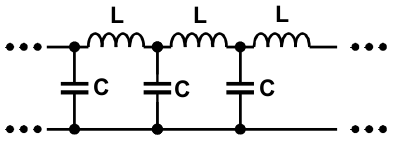
\includegraphics[height=2.5cm]{Tiefpass.png}
    \caption{Tiefpass \cite{anleitung}.}
    \label{subfig:Tiefpass}
  \end{subfigure}
  \begin{subfigure}{0.48\textwidth}
    \centering
    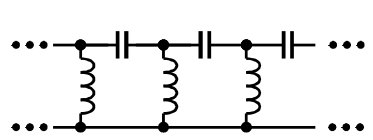
\includegraphics[height=2.5cm]{Hochpass.png}
    \caption{Hochpass \cite{anleitung}.}
    \label{subfig:Hochpass}
  \end{subfigure}
  \caption{verschiedene Kettenschaltungen \cite{anleitung}.}
  \label{fig:Ketten}
\end{figure}

Im Folgenden werden LC-Ketten mit konstanten und
alternierenden Kapazitäten analysiert.


\subsection{Dispersionsrelation einer LC-Kettenschaltung}

Über die Kirchhoffschen Gesetze kann mit Hilfe der in Abbildung
\ref{fig:KetteLC} dargestellten Ströme und Spannungen die Schwingungsgleichung
einer LC-Kettenschaltung aufgestellt werden.

\begin{figure}
  \centering
  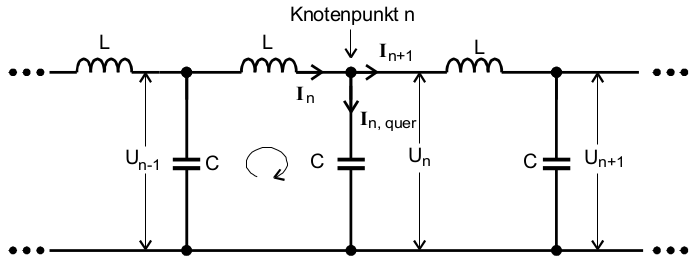
\includegraphics[height=4cm]{KetteLC.png}
  \caption{Ströme und Spannungen in einer LC-Kette \cite{anleitung}.}
  \label{fig:KetteLC}
\end{figure}

Aus der Knotenregel

\begin{equation}
  \sum_{n} I_n = 0
  \label{eqn:Knoten}
\end{equation}
folgt

\begin{equation}
  I_n - I_{n+1} - I_{n,\text{quer}} = 0
\end{equation}
und aus der Maschenregel

\begin{equation}
  \sum_{n} U_n = 0
  \label{eqn:Masche}
\end{equation}
im eingeschwungenen Zustand

\begin{equation}
  I_{n} = \frac{U_{n} - U_{n-1}}{\symup{i} \omega L}
\end{equation}
und

\begin{equation}
  I_{n,\text{quer}} = U_{n} \symup{i} \omega C.
\end{equation}
Daraus folgt durch Einsetzen und Umformen die Schwingungsgleichung

\begin{equation}
  \frac{U_{n} - U_{n-1}}{\symup{i} \omega L} - \frac{U_{n+1} - U_{n}}{\symup{i}
  \omega L} - \symup{i} U_{n} \omega C = 0,
\end{equation}
die mit dem Ansatz

\begin{equation}
  U_{n}(t) = U_0 \symup{e}^{\symup{i}t (\omega - n \theta)}
\end{equation}
gelöst werden kann.
Es ergibt sich die Dispersionsrelation

\begin{equation}
  \omega_k(\theta) = \sqrt{\frac{2}{LC}(1-\cos\theta)},
  \label{eqn:Dispersion}
\end{equation}
das ist die Kreisfrequenz
$\omega_k$ in Abhängigkeit von der Phasenverschiebung $\theta$ pro Kettenglied.
Der maximale Wert für $\omega_k$ ist die Grenzfrequenz $\bar{\omega}$
mit

\begin{equation}
  \bar{\omega} = \sqrt{\frac{2}{LC}}.
\end{equation}
Hochfrequentere Schwingungen werden von dem Tiefpass herausgefiltert.


\subsection{Dispersionsrelation einer alternierenden LC-Kettenschaltung}

Mit einer alternierenden LC-Kettenschaltung ist hier ein Tiefpass gemeint,
bei dem zwei unterschiedliche Kapazitäten $C_1$ und $C_2$ alternierend
parallel in die Schaltung eingebaut werden. Dies ist in Abbildung
\ref{fig:KetteLC1C2} dargestellt.

\newpage

\begin{figure}
  \centering
  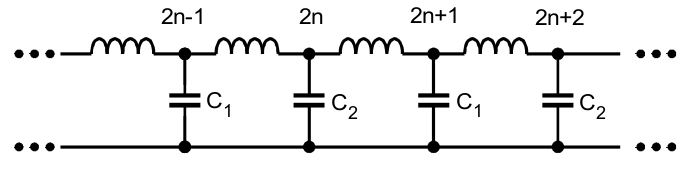
\includegraphics[height=3cm]{KetteLC1C2.png}
  \caption{Knotenpunkte in einer alternierenden LC-Kette \cite{anleitung}.}
  \label{fig:KetteLC1C2}
\end{figure}

Aus den Kirchhoffschen Gesetzen \eqref{eqn:Knoten} und \eqref{eqn:Masche}
folgen für diese Schaltung zwei Schwingungsgleichungen

\begin{equation}
  -\omega^2 C_1 U_{2n+1} + \frac{1}{L}(-U_{2n}+2U_{2n+1}-U_{2n+2}) = 0
\end{equation}
und

\begin{equation}
  -\omega^2 C_2 U_{2n} + \frac{1}{L}(-U_{2n+1}+2U_{2n+1}-U_{2n+1}) = 0.
\end{equation}
Durch Einsetzen der Lösungsansätze

\begin{equation}
  U_{2n+1} = U_{0_1} \symup{e}^{\symup{i(\omega t + (2n+1)\theta)}}
\end{equation}
und

\begin{equation}
  U_{2n} = U_{0_2} \symup{e}^{\symup{i(\omega t + 2n\theta)}}
\end{equation}
ergibt sich die Koeffizientenmatrix

\begin{equation}
  \symbf{M} =
  \begin{pmatrix}
    -\omega^2 C_1 + \frac{2}{L} & -\frac{2}{L} \cos \theta \\
    -\frac{2}{L} \cos \theta & -\omega^2 C_2 + \frac{2}{L}
  \end{pmatrix}
  \label{eqn:Matrix}
\end{equation}
mit

\begin{equation}
  \symbf{M} \cdot \vec{U_0} = \vec{0}.
\end{equation}
Um eine nicht-triviale lösung zu erhalten, muss das charakteristische Polyom,
also die Determinante der Matrix \eqref{eqn:Matrix}, Null sein.
Es folgt

\begin{equation}
  \omega^4 - \omega^2 \frac{2}{L} \biggl(\frac{1}{C_1} + \frac{1}{C_2}\biggr)
  \frac{4}{L^2 C_1 C_2} (1 - \cos^2 \theta) = 0
\end{equation}
und daraus zwei sinnvolle Lösungen für die Kreisfrequenz \omega

\begin{equation}
  \omega_1, \omega_2 (\theta) = \sqrt{\frac{1}{L} \biggl(\frac{1}{C_1} +
  \frac{1}{C_2}\biggr)
  \pm \frac{1}{L} \sqrt{\biggl(\frac{1}{C_1} + \frac{1}{C_2}\biggr)^2 -
  \frac{4 \sin^2 \theta}{C_1C_2}}}.
  \label{eqn:Omega}
\end{equation}
Die beiden resultierenden Kurvenäste sind in Abbildung \ref{fig:KurveLC1C2}
dargestellt.

\begin{figure}
  \centering
  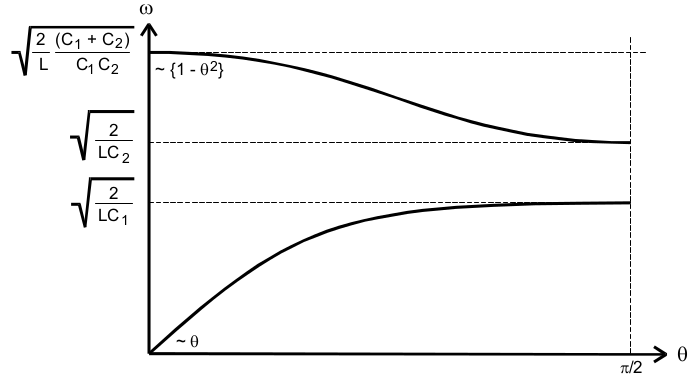
\includegraphics[height=7cm]{KurveLC1C2.png}
  \caption{Skizze der Graphen von $\omega_1$ und $\omega_2$.}
  \label{fig:KurveLC1C2}
\end{figure}

Bei dem unteren Kurvenast $\omega_1$ mit negativem Vorzeichen vor der Wurzel
in Gleichung \eqref{eqn:Omega}
steigt die Kreisfrequenz zunächst annähernd konstant an und kann für kleine
\theta durch die Gleichung

\begin{equation}
  \omega_1 (\theta) = \sqrt{\frac{2}{L(C_1 + C_2)}} \theta
\end{equation}
beschrieben werden.
Die Funktion erreicht ihren Maximalwert bei $\frac{\pi}{2}$ an
der ersten Grenzfrequenz

\begin{equation}
  \omega_1\Bigl(\frac{\pi}{2}\Bigr) = \bar{\omega}_a = \sqrt{\frac{2}{LC_1}}.
\end{equation}
Bei dem oberen Kurvenast $\omega_2$ mit positivem Vorzeichen vor der Wurzel in
Gleichung \eqref{eqn:Omega} ist die Funktion zunächst annähernd
proportional zu $(1-\theta^2)$.
Sie hat ein Minimum bei der zweiten Grenzfrequenz

\begin{equation}
  \omega_2\Bigl(\frac{\pi}{2}\Bigr) = \bar{\omega}_b = \sqrt{\frac{2}{LC_2}}
\end{equation}
und ein Maximum bei der dritten Grenzfrequenz

\begin{equation}
  \omega_2(0) = \bar{\omega}_c = \sqrt{\frac{2(C_1+C_2)}{LC_1C_2}}.
\end{equation}
Zwischen den Grenzfrequenzen $\bar{\omega}_a$ und $\bar{\omega}_b$ und ab der
oberen Grenzfrequenz $\bar{\omega}_c$ werden alle Frequenzen durch den
Tiefpass herausgefiltert. Die restlichen Frequenzen, die im Wertebereich der
Funktionen $\omega_1$ und $\omega_2$ liegen, werden nicht herausgefiltert.


\subsection{Phasen- und Gruppengeschwindigkeit einer LC-Kettenschaltung}

Die Phasengeschwindigkeit einer Welle ist die Zeit $t$, die eine
Phasenverschiebung $\theta$ benötigt, um eine bestimmt Strecke zurückzulegen.
In einer Kettenschaltung wird die Strecke durch die Menge an zurückgelegten
Kettengliedern $n$ beschrieben.
Für die allgemeine Phasengeschwindigkeit in der LC-Kette folgt daher

\begin{equation}
  v_\text{ph} = \frac{\Delta n}{\Delta t} = \frac{\omega}{\theta}.
  \label{eqn:Phase}
\end{equation}
Bei dieser Phasengeschwindigkeit wird von einer harmonischen Welle ausgegangen.
Bei einer sogenannten Wellengruppe, die in Abbildung \ref{fig:WP} dargestellt
ist, verhält sich die Phasengeschwindigkeit gleich, es existiert aber zusätzlich
eine sogenannte Gruppengeschwindigkeit.

\begin{figure}
  \centering
  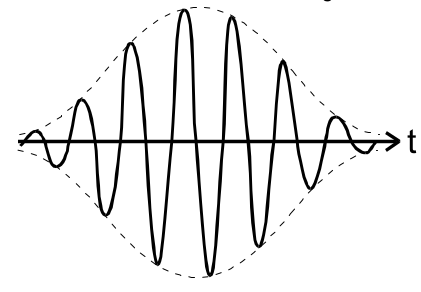
\includegraphics[height = 3.5cm]{Wellengruppe.png}
  \caption{Graphische Darstellung eines Wellenpaketes \cite{anleitung}.}
  \label{fig:WP}
\end{figure}

Nach Gleichung \eqref{eqn:Phase}
muss diese Welle frequenzabhängig sein, was zur Folge hat, dass auch die
Phasengeschwindigkeit $v_\text{ph}$ in der LC-Kette von der Frequenz abhängen
muss.
Über die bereits berechnete Dispersionsrelation \eqref{eqn:Dispersion} einer
LC-Kette kann die Phasengeschwindigkeit bestimmt werden.
Sie lautet

\begin{equation}
  v_\text{ph} = \frac{\omega}{\theta} = \frac{\omega}{\arccos \Bigl(
  1-\frac{1}{2}\omega^2LC\Bigr)}.
\end{equation}
Die einzelnen Fourierkomponenten der Welle haben wie bereits erwähnt
unterschiedliche Phasengeschwindigkeiten, weshalb die Wellengruppe sich in Zeit
und Raum ausdehnt. Die erwähnte Gruppengeschwindigkeit ist die
Ausdehnungsgeschwindigkeit des Wellengruppenmaximums.
Durch Überlagerung zweier Wellen mit ähnlichen Frequenzen können Wellengruppen
erzeugt werden. Diese Überlagerung nennt man Schwebung. Sie ist in Abbildung
\ref{fig:Schweb} dargestellt.

\begin{figure}
  \centering
  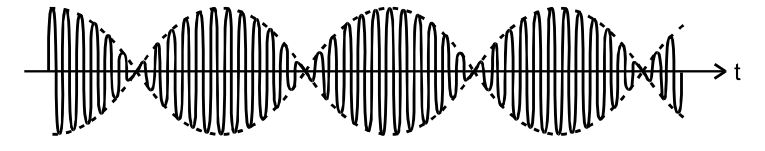
\includegraphics[height = 2.5cm]{Schwebung.png}
  \caption{Überlagerung von zwei ähnlichen Wellen \cite{anleitung}.}
  \label{fig:Schweb}
\end{figure}

Für die Berechnung der Gruppengeschwindigkeit der Wellengruppen einer Schwebung
kann angenommen werden, dass

\begin{align}
\frac{1}{2}(\omega + \omega') & = \omega & \frac{1}{2}(\theta + \theta') &
= \theta
\label{eqn:SchwebungBedingung}
\end{align}
ist, da die Wellen zunächst ähnlich sein müssen.
Die Amplituden der beiden Wellen seien ebenfalls ähnlich und es gilt

\begin{equation}
  A(t) = A_0 \Bigl(\cos(\omega t - \theta) \cos(\omega' t - \theta')\Bigr).
\end{equation}
Mit Hilfe der trigonometrischen Additionstheoreme und den Annahmen aus den
Gleichungen \eqref{eqn:SchwebungBedingung} folgt

\begin{equation}
  A(t) = 2 A_0 \cos(\omega t - \theta) \cdot \cos \Bigr(\frac{1}{2}
  ((\omega-\omega')t-(\theta-\theta'))\Bigr).
\end{equation}
mit der Amplitude

\begin{equation}
  \cos \Bigr(\frac{1}{2}
  ((\omega-\omega')t-(\theta-\theta'))\Bigr).
\end{equation}
Die Gruppengeschwindigkeit beträgt nun

\begin{equation}
  v_\text{gr} = \frac{\omega - \omega'}{\theta - \theta'} =
  \frac{\symup{d}\omega}{\symup{d}\theta} =
  \frac{1}{\sqrt{LC}}\sqrt{1 - \frac{1}{4}LC\omega^2}
\end{equation}
Für kleine Frequenzen $\omega \to 0$ nähern sich sowohl die Phasen- als auch
die Gruppengeschwindigkeit dem Wert $\sqrt{\frac{1}{LC}}$ an.
Für Frequenzen $\omega > \frac{2}{\sqrt{LC}}$  ist die
Gruppengeschwindigkeit

\begin{equation}
  v_\text{gr} = 0.
\end{equation}

\subsection{Der Wellenwiderstand einer unendlichen LC-Kette}

Der Eingangswiderstand, oder auch Wellenwiderstand $Z$ ist der Widerstand, der
bei einer theoretischen unendlichen Kette existiert.
Er ist der Quotient aus der Eingangsspannung und dem Eingangsstrom.
Nach Abbildung \ref{fig:WW} kann mit Hilfe der Kirchhoffschen Gesetze die
Gleichung

\begin{equation}
  I_0 - \symup{i}\omega \frac{C}{2} U_0 + \frac{U_1 - U_0}{\symup{i}\omega L}=0
  \label{eqn:Eingang}
\end{equation}
aufgestellt werden.

\newpage

\begin{figure}
  \centering
  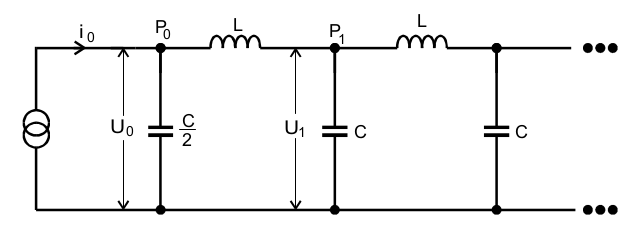
\includegraphics[height = 4cm]{Wellenwiderstand.png}
  \caption{Berechnung der Eingangsimpedanz \cite{anleitung}.}
  \label{fig:WW}
\end{figure}

Mit dem Lösungsansatz

\begin{equation}
  U_n(\theta) = U_0 \symup{e}^{-\symup{i}n\theta}
\end{equation}
für das $n$-te Kettenglied und der Dispersionsrelation \eqref{eqn:Dispersion}
kann die Gleichung \eqref{eqn:Eingang} zu

\begin{equation}
  Z = \frac{U_0}{I_0} = \frac{\omega L}{\sin \theta}
\end{equation}
und schließlich zum Wellenwiderstand in Abhängigkeit von $\omega$

\begin{equation}
  Z(\omega) = \sqrt{\frac{L}{C}} \frac{1}{\sqrt{1-\frac{1}{4}\omega^2 LC}}.
  \label{eqn:Zfuerunendlich}
\end{equation}
umgeformt werden.
Wie an Gleichung \eqref{eqn:Zfuerunendlich} erkennbar ist, ist der
Wellenwiderstand reell, womit die Stromstärke und Spannung in Phase sind.
Eine unendliche LC-Kette ist nicht realisierbar, zur Simulation kann
allerdings eine endliche LC-Kette verwendet werden, in welcher der
Wellenwiderstand an das Ende der Kette geschaltet wird wie in Abbildung
\ref{fig:endK}.

\begin{figure}
  \centering
  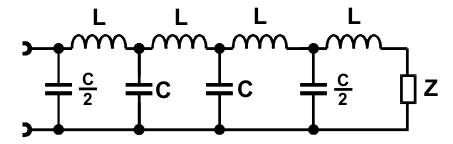
\includegraphics[height = 2.5cm]{endlicheWelle.png}
  \caption{Wellenwiderstand $Z$ in einer endlichen Kette \cite{anleitung}.}
  \label{fig:endK}
\end{figure}

Eine Skizze von $Z(\omega)$ ist in Abbildung \ref{fig:WO} abgebildet. Da der
Wellenwiderstand für Frequenzen, die deutlich unter der Grenzfrequenz
$\bar{\omega}$ liegen, annähernd konstant ist, kann dieser mit dem Grenzwert
des Wertebereichs

\begin{equation}
  \omega = \sqrt{\frac{1}{LC}}
  \label{eqn:WaveWiderstand}
\end{equation}
eingebaut werden.

\begin{figure}
  \centering
  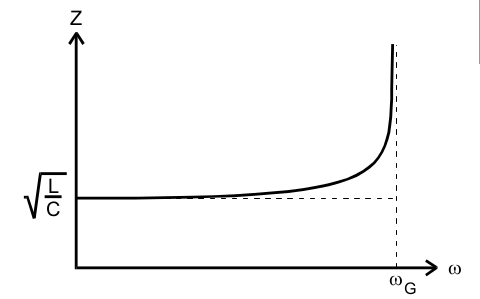
\includegraphics[height = 5cm]{WiderstandOmega.png}
  \caption{Skizze des Wellenwiderstandes $Z$ in Abhängigkeit von $\omega$
  \cite{anleitung}.}
  \label{fig:WO}
\end{figure}


\subsection{Eigenschaften einer endlichen LC-Kette}

Bei einer endlichen LC-Kette werden die Signale am Kettenende reflektiert.
Aufrgrund der Überlagerung von hin- und rücklaufenden Wellen können
stehende Wellen entstehen.
Zunächst wird der Quotient der Amplituden beider Wellen gebildet, wobei davon
ausgegangen wird, dass am Ende der Kettenschaltung ein komplexer Widerstand
$r$ geschaltet ist, der eine Phasenverschiebung und Abschwächung der
hinlaufenden Welle bewirken kann.
In Abbildung \ref{fig:Abschluss} sind die Ströme und Spannungen am Kettenende
dargestellt.

\begin{figure}
  \centering
  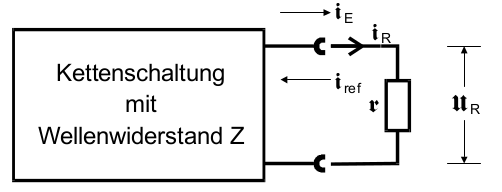
\includegraphics[height = 3.5cm]{Abschlusswiderstand.png}
  \caption{Ströme und Spannungen am Kettenende einer endlichen LC-Kette
  \cite{anleitung}.}
  \label{fig:Abschluss}
\end{figure}

Für die Spannung am Abschlusswiderstand gilt

\begin{equation}
  U_\text{R} = U_\text{E} + U_\text{ref}
\end{equation}
und für die Stromstärke äquivalent

\begin{equation}
  I_\text{R} = I_\text{E} + I_\text{ref}.
\end{equation}
Wegen des Ohmschen Gesetzes

\begin{equation}
  U = RI
\end{equation}
gilt für die Abschlussspannung

\begin{equation}
  U_\text{R} = I_\text{R} r,
\end{equation}
für den hinlaufenden Strom

\begin{equation}
  I_\text{E} = \frac{U_\text{E}}{Z}
\end{equation}
mit dem Wellenwiderstand $Z$ der Kette und für den reflektierten Strom

\begin{equation}
  I_\text{ref} = - \frac{U_\text{ref}}{Z}.
\end{equation}
Daraus folgt das Spannungsverhältnis

\begin{equation}
  \frac{U_\text{ref}}{U_\text{E}} = \frac{r-Z}{r+Z}.
\end{equation}
Es werden nun drei Spezialfälle behandelt.
Strebt $r \to \infty$, existiert also ein offenes Ende, so gilt die Gleichung

\begin{equation}
  U_\text{ref} = U_\text{E}.
\end{equation}
In diesem Fall wird die Welle also total ohne Phasenverschiebung reflektiert.
Die Superposition der hin- und rücklaufenden Wellen mit

\begin{align}
  A_\text{hin} & = A_0 \cos(\omega t - n \theta) &
  A_\text{rück} & = A_0 \cos(\omega t + n \theta)
\end{align}
ist

\begin{equation}
  A_\text{sup,1} =  2A_0 \cos \omega t \cos n \theta.
\end{equation}
Es kann sich eine stehende Welle ausbilden, falls am Kettenende ein
Spannungsbauch auftritt, also wenn

\begin{equation}
  n_\text{max}\theta_\text{k} = k \pi
  \label{eqn:BauchKnoten}
\end{equation}
mit $k \in \mathbb{Z}$. Dies ist in Abbildung \ref{fig:BauchKnot} abgebildet.
Ist der Abschlusswiderstand $r = 0$, was bei einer kurzgeschlossenen Kette
der Fall ist, so gilt

\begin{equation}
  U_\text{ref} = -U_\text{E}
\end{equation}
In diesem Fall wird die Welle total mit einer Phasenverschiebung $\pi$
reflektiert.
Die Superposition der hin- und rücklaufenden Wellen mit

\begin{align}
  A_\text{hin} & = A_0 \cos(\omega t - n \theta) &
  A_\text{rück} & = -A_0 \cos(\omega t + n \theta)
\end{align}
ist

\begin{equation}
  A_\text{sup,2} =  2A_0 \sin \omega t \sin n \theta.
\end{equation}
Es kann sich eine stehende Welle ausbilden, falls am Kettenende ein
Spannungsknoten auftritt, also ebenfalls wenn Gleichung
\eqref{eqn:BauchKnoten} gilt.
Auch dieser Fall ist in Abbildung \ref{fig:BauchKnot} abgebildet.

\begin{figure}
  \centering
  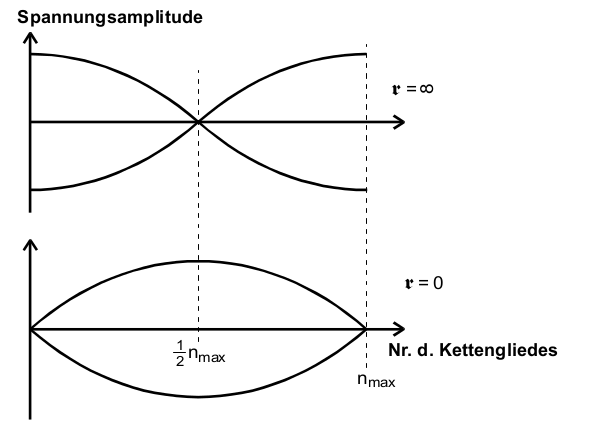
\includegraphics[height = 7.5cm]{Reflexion.png}
  \caption{Spannungsamplitude einer stehenden Welle \cite{anleitung}.}
  \label{fig:BauchKnot}
\end{figure}

Der letzte Fall $r=Z$, welcher eine unendliche Kette beschreibt, wurde bereits
behandelt. Die Welle wird nicht reflektiert, es gilt

\begin{equation}
  U_\text{ref} = 0.
\end{equation}
